\documentclass[border=10pt]{standalone}

\usepackage{tikz}
\usepackage{tikzsymbols}
\usetikzlibrary{calc,patterns,shapes.geometric}

\def\centerarc[#1](#2)(#3:#4:#5){\draw[#1] ($(#2)+({#5*cos(#3)},{#5*sin(#3)})$) arc (#3:#4:#5);}

\begin{document}
	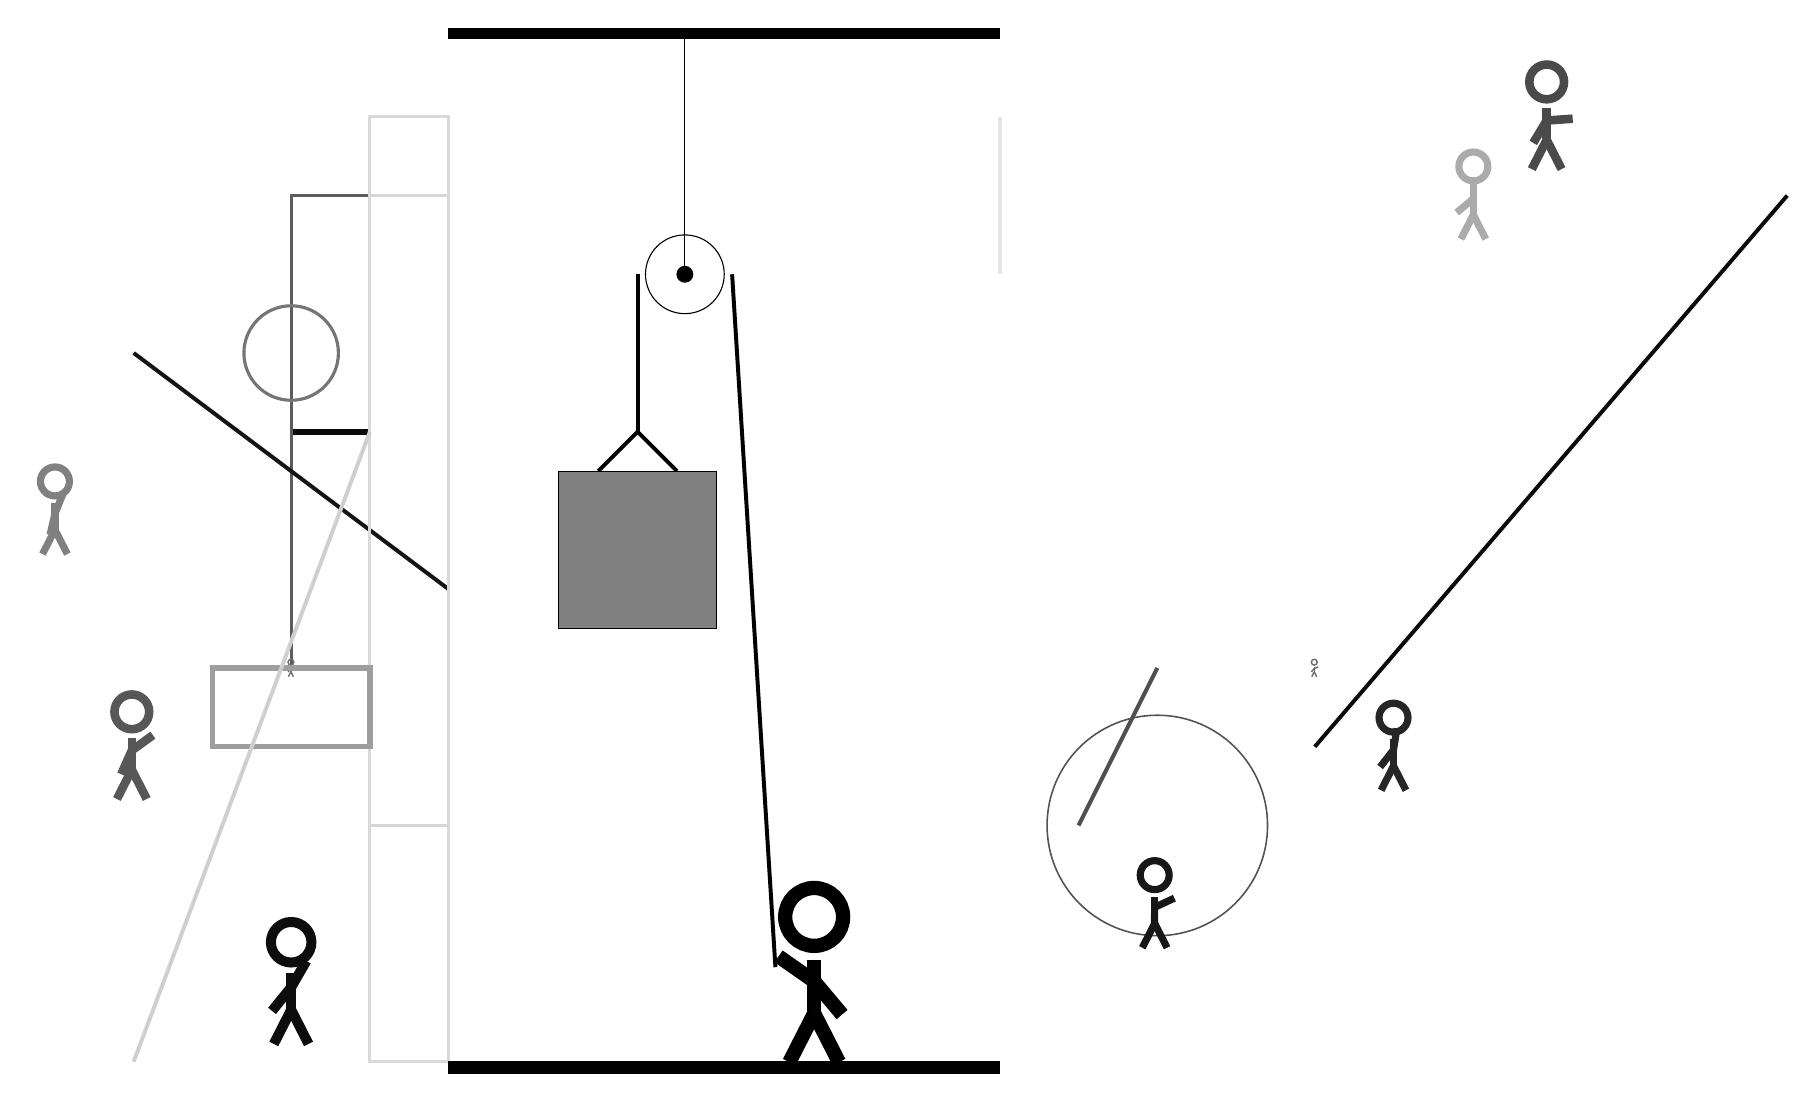
\begin{tikzpicture}
		%%%%% START %%%%%
		
		\draw[fill=black] (-2, 10) rectangle (5, 10.125);
		
		\draw (1, 7) circle (0.5);
		\draw[fill=black] (1, 7) circle (0.1);
		\draw (1, 10) -- (1, 7);
		
		\draw[line width=0.5mm] (-0.1, 4.5) -- (0.4, 5.0) -- (0.9, 4.5);
		\draw[fill=black!50] (-0.6, 4.5) rectangle (1.4, 2.5);
		
		\draw[line width=0.5mm] (0.4, 7) -- (0.4, 5.0);
		\centerarc[line width=0.5mm](1, 7)(0:180:0.6);
		\draw[line width=0.5mm](1.6, 7) -- (2.15, -1.8);
		
		\node at (2.6, -1.9) {\Strichmaxerl[10][-35][-50]};
		
		\node[line width=0.7mm, color=black!57] at (9, 2) {\Strichmaxerl[1][49][24]};
		
		\draw[line width=0.7mm, color=black!96] (-3, 5) rectangle (-4, 5);
		\node[line width=0.5mm, color=black!50] at (-7, 4) {\Strichmaxerl[5][77][68]};
		\draw[line width=0.5mm, color=black!10](5, 9) -- (5, 7);
		\draw[line width=0.4mm, color=black!64] (-4, 8) rectangle (-3, 2);
		\node[line width=0.6mm, color=black!66] at (-6, 1) {\Strichmaxerl[6][66][36]};
		\draw[line width=0.5mm, color=black!92](-6, 6) -- (-2, 3);
		\node[line width=0.7mm, color=black!33] at (11, 8) {\Strichmaxerl[5][40][90]};
		\node[line width=0.5mm, color=black!56] at (-4, 2) {\Strichmaxerl[1][50][38]};
		\node[line width=0.5mm, color=black!85] at (10, 1) {\Strichmaxerl[5][52][81]};
		\draw[line width=0.3mm, color=black!16] (-3, 0) rectangle (-2, 8);
		
		\draw [line width=0.2mm, color=black!68](7, 0) circle (1.4);
		\draw[line width=0.4mm, color=black!15] (-2, -3) rectangle (-3, 9);
		\node[line width=0.4mm, color=black!71] at (12, 9) {\Strichmaxerl[6][59][4]};
		\draw[line width=0.5mm, color=black!69](7, 2) -- (6, 0);
		\draw[line width=0.5mm, color=black!96](9, 1) -- (15, 8);
		\draw[line width=0.7mm, color=black!38] (-3, 1) rectangle (-5, 2);
		\draw [line width=0.4mm, color=black!54](-4, 6) circle (0.6);
		\node[line width=0.2mm, color=black!91] at (7, -1) {\Strichmaxerl[5][89][25]};
		
		\draw[line width=0.5mm, color=black!19](-3, 5) -- (-6, -3);
		\node[line width=0.2mm, color=black!95] at (-4, -2) {\Strichmaxerl[7][51][60]};
		
		
		\draw[fill=black] (-2, -3) rectangle (5, -3.15);
		
		%%%%% END %%%%%
	\end{tikzpicture}
\end{document}